\documentclass[../main.tex]{subfiles}
\graphicspath{{\subfix{../img/}}}
\begin{document}

\newpage
\section{Lösungskonzept}

In diesem Kapitel wird das gewählte Lösungskonzept ''Simpel'' (siehe Anhang \ref{a3:loesungsvariante_Simpel}) näher erläutert. Wieso das Lösungskonzept ''Beweglich'' ausgeschieden ist, lese im Anhang \ref{a3:EntscheidLösungsvariante}. Bei dem gewählten Konzept liegt der Schwerpunkt auf einer möglichst einfachen Lösung, da ein einfach konstruiertes System in der Regel robuster im Einsatz ist. Im folgenden Text wird für jede Teilfunktion die einfachste Lösung erarbeitet und beschrieben.

\begin{figure}[H]
\centering
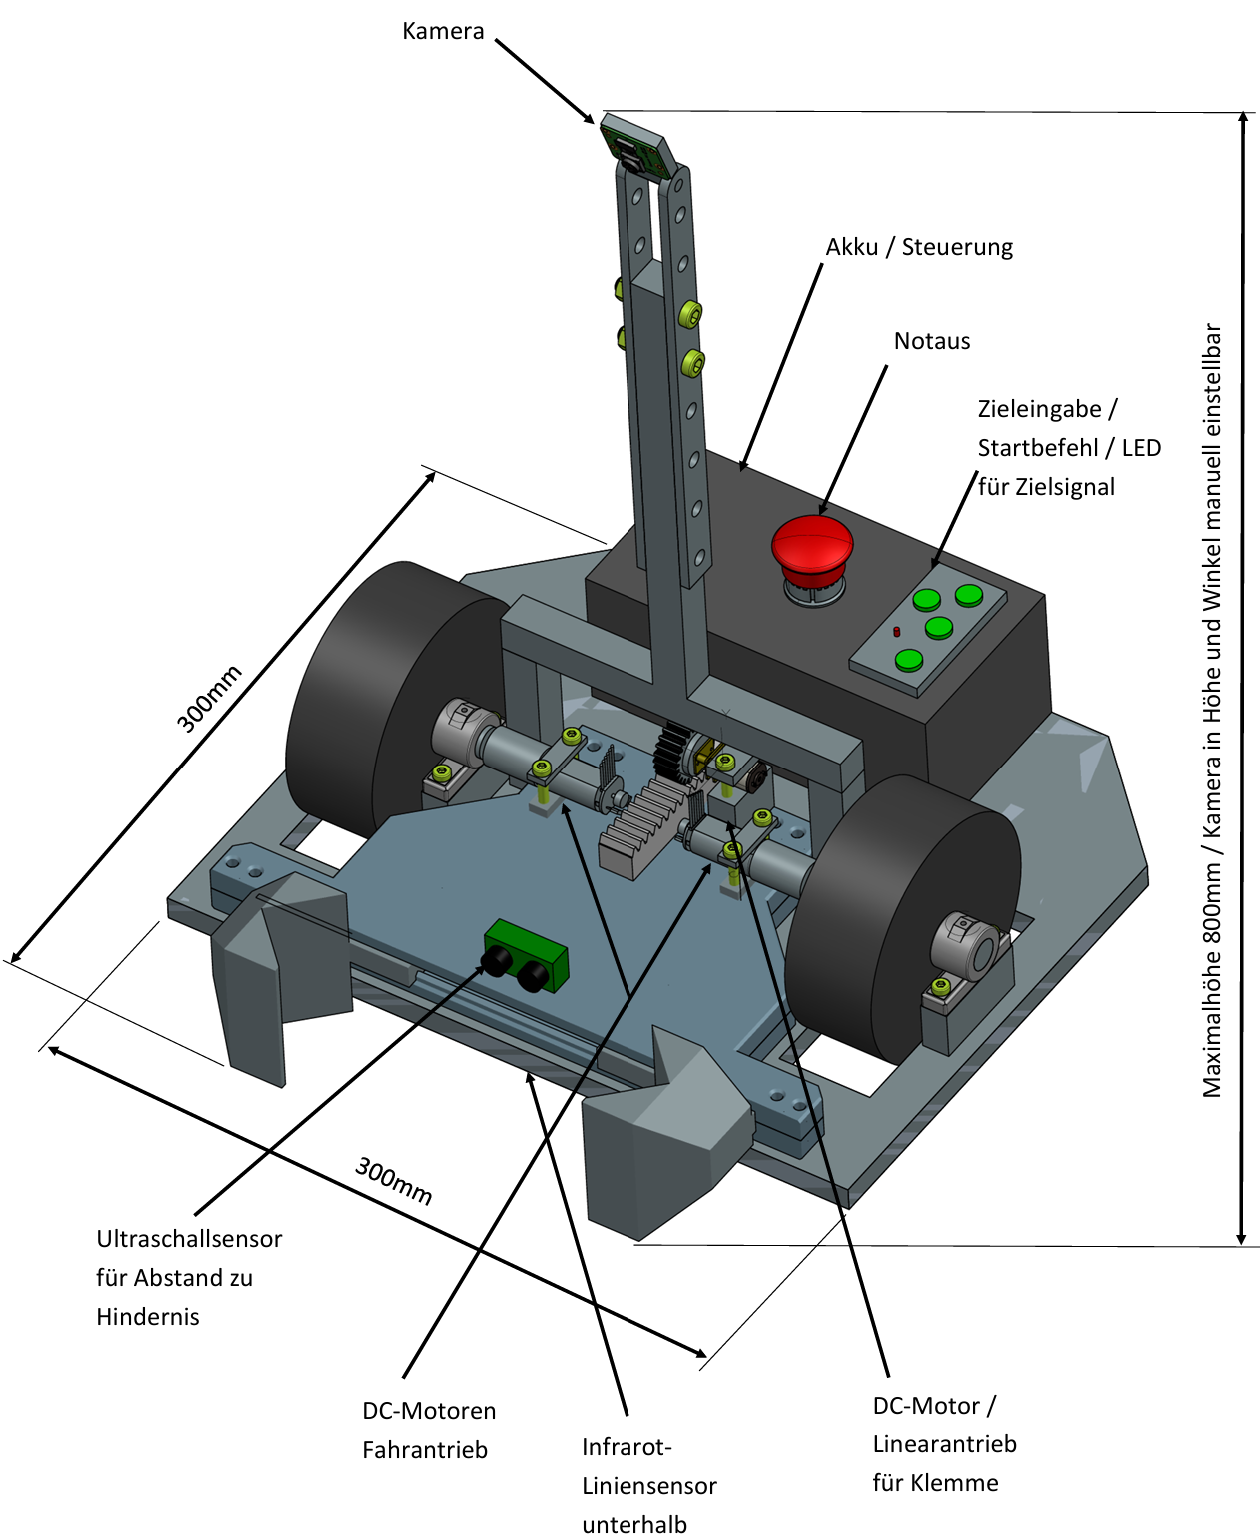
\includegraphics[width=0.85\linewidth]{Skizze Konzept beschriftet.png}
\caption{Konzept-Skizze Fahrzeug}
\label{img:Konzept-Skizze_Fahrzeug}
\end{figure}

\subsection{Ablauf}

Im Ablaufdiagramm (Abbildung \ref{img:ablaufdiagramm}) wird der Ablauf des Roboters von Start bis Ziel übersichtlich aufgezeigt.

\begin{figure}[H]
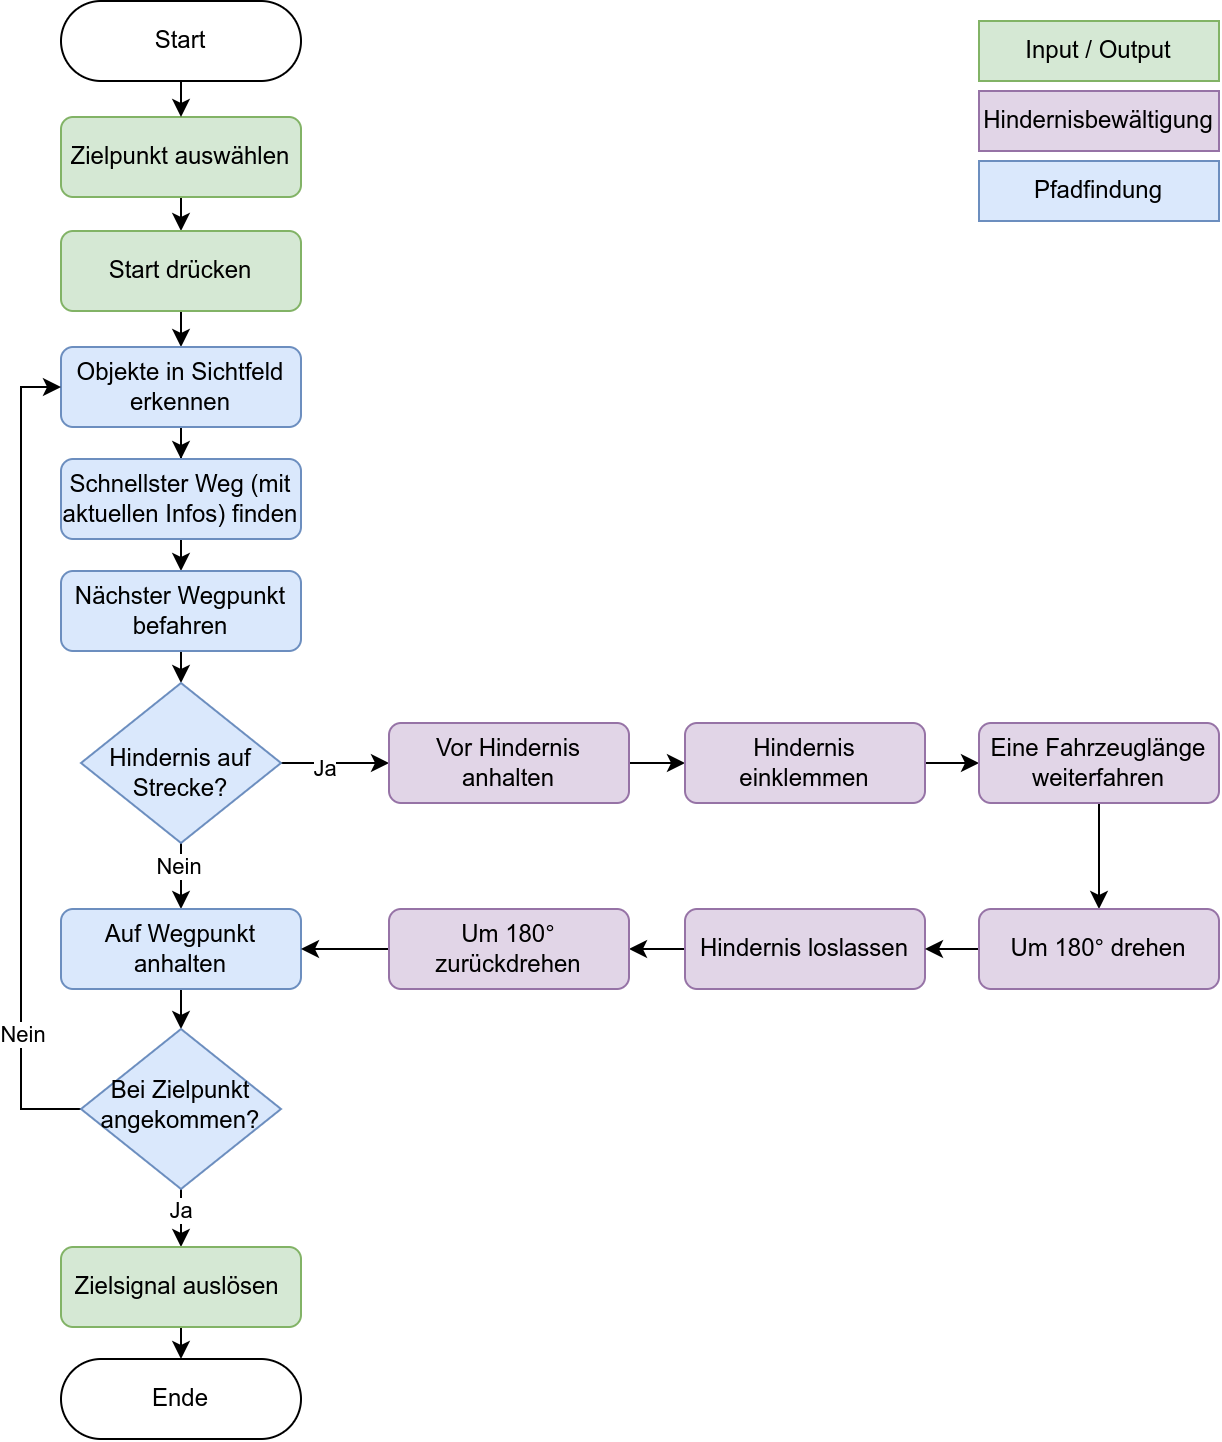
\includegraphics[width=0.9\textwidth]{img/lösungskonzpet/Ablaufdiagramm.png}
\caption{Ablaufdiagramm}
\label{img:ablaufdiagramm}
\end{figure}

\subsection{Objekterkennung} %Objekterekennung, idealer Weg, 
Die Objekterkennung wird mithilfe eines Raspberry Pi und der dazugehörigen Pi-Kamera durchgeführt. Dabei werden Pylonen, Hindernisse und Wegpunkte erkannt. Als Software kommt YOLO zum Einsatz (Anhang \ref{a3:Objekterkennung}. Diese Daten werden dann für die Wegfindung genutzt. Das Ziel ist, möglichst viel des Graphen zu erfassen und auszuwerten. Gelingt dies nicht, wird am nächsten Punkt eine weite Objektkennung durchgeführt. 

\subsection{Wegfindungssoftware}

Um den schnellsten Weg ins Ziel zu finden, wird der Graph in der Software abgespeichert
und der kürzeste Weg mittels Dijkstra Algorithmus berechnet(Anhang \ref{a3:Wegfindung}. Sobald neue Informationen der Strecke erkannt werden, wird der Graph entsprechend angepasst und der kürzeste Weg wird anhand der aktuellen Position neu ermittelt.
Ursprünglich haben alle Linien im Graphen eine einheitliche Gewichtung. 

Je nach neu erhaltener Information werden andere Anpassungen am Graphen vorgenommen:
\begin{itemize}
    \item Pylon auf Wegpunkt erkannt: Wegpunkt (Knote) wird aus dem Graphen entfernt
    \item Linie wurde entfernt: Linie (Kante) wird aus dem Graphen entfernt.
    \item Hindernis auf Linie erkannt: Linie (Kante) erhält mehr Gewichtung.
\end{itemize}

\subsection{Fortbewegung} 

Die Fortbewegung wird nach dem Prinzip Roomba realisiert. Wie der Name schon erahnen lässt, handelt es sich dabei um ein ähnliches System, wie wir es von Staubsauger-Robotern kennen. Das Prinzip besteht aus zwei einzeln angetriebenen Rädern und einem Stützelement. Die angetriebenen Räder können unabhängig in beide Drehrichtungen angetrieben werden, wodurch ein Wenden an Ort und Stelle ermöglicht wird. Die beiden Räder sind in Längsrichtung zentrisch angeordnet, damit sich das Fahrzeug um den eigenen Mittelpunkt drehen kann, ohne dass ein Versatz entsteht. Weitere Details dazu befinden sich im Anhang unter \ref{a3:}

Als Antriebsmotoren werden Brushed-DC-Motoren verwendet, die über eine H-Brücke mit einem PWM-Signal angesteuert werden können. Jeder Motor verfügt über einen Encoder, der überwacht, dass beide Motoren die gleiche Anzahl an Umdrehungen ausführen. Gesteuert werden die Motoren von einem TinyK22 (wieso der TinyK22 gewählt wurde, siehe Anhang \ref{a3:Hardware Steuerung}), der die H-Brücke ansteuert. Weitere Details können im Anhang, unter \ref{a3:Fahrantrieb} und \ref{a3:Sensorik:Positionsabfrage} nachgeschlagen werden.
\newpage
Der TinyK22 ist über eine UART-Schnittstelle mit dem Raspberry Pi verbunden (siehe Abbildung \ref{img:UART_Schnittstelle}). Zunächst sendet der TinyK22 das gewünschte Ziel an den Raspberry Pi. Der Raspberry Pi wertet mit der Kamera aus, welches der nächste beste Punkt ohne Pylone ist und teilt anschliessend dem TinyK22 mit, um welchen Winkel das Fahrzeug ausgerichtet werden muss, um diesen Punkt zu erreichen. Somit dreht sich das Fahrzeug auf die angepeilte Linie, dies wird vom Liniensensor darauf erkannt. Wird die Linie nicht erkannt, sucht das System diese durch Drehungen im Bereich von ±15 Grad. Sobald die Linie gefunden wird, meldet der TinyK22 dem Raspberry Pi, wie weit sich das Fahrzeug gedreht hat.

\begin{figure}[H]
\centering
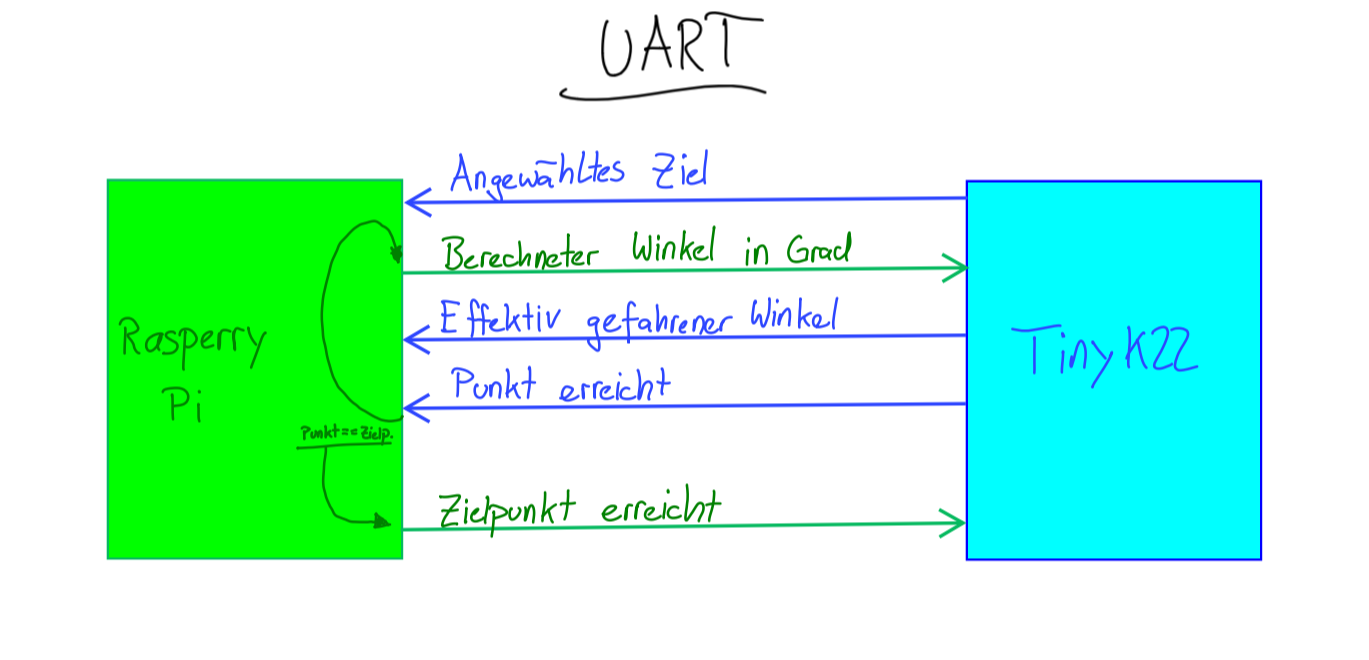
\includegraphics[width=0.7\textwidth]{img/lösungskonzpet/Skizzen/UART_Schnittstelle.png}
\caption{UART Schnittstelle}
\label{img:UART_Schnittstelle}
\end{figure}

Das Fahrzeug folgt der Linie mithilfe des Liniensensors. Erkennt der Sensor eine breitere Linie, also einen Punkt, informiert der TinyK22 den Raspberry Pi, stoppt das Fahrzeug, und der Vorgang beginnt erneut. Sobald das Fahrzeug den Zielpunkt erreicht, signalisiert der Raspberry Pi dies dem TinyK22, der daraufhin eine LED blinken lässt.

\newpage

\subsection{Hindernisbewältigung} %Hindernisvermessung, Antrieb, Mechanik,
Der Ultraschallsensor überwacht kontinuierlich, ob sich ein Hindernis auf der Linie befindet (siehe Anhang \ref{a3:Objekterkennung_Sensor}). Sobald ein Hindernis in 30 cm Entfernung detektiert wird, verlangsamt sich das Fahrzeug und fährt langsam darauf zu, bis es zwischen den zwei seitlichen Klemmbacken positioniert ist. Diese Distanz ist vorprogrammiert, und das Fahrzeug hält an. Danach wird der Schrittmotor angesteuert, der das Hindernis ergreift und mit einem Mechanismus anhebt (Anhang \ref{a3:Hindernisbewältigungsantrieb} und \ref{a3:Aufnahme_Hindernis}).
Das Fahrzeug fährt anschliessend eine Fahrzeuglänge vor, wobei die Encodermessung die Distanz überwacht. Danach dreht es sich um 180 Grad, und der Schrittmotor löst die Klemmen. Das Fahrzeug fährt nun ein Stück zurück, um das Hindernis nicht mehr zwischen den Klemmbacken zu haben, und vollzieht eine weitere 180-Grad-Drehung. Abschliessend fährt das Fahrzeug mithilfe des Liniensensors entlang der Linie zum nächsten Punkt(siehe Abbildung \ref{img:Skizze_Hindernisbewältigung}.

\begin{figure}[H]
\centering
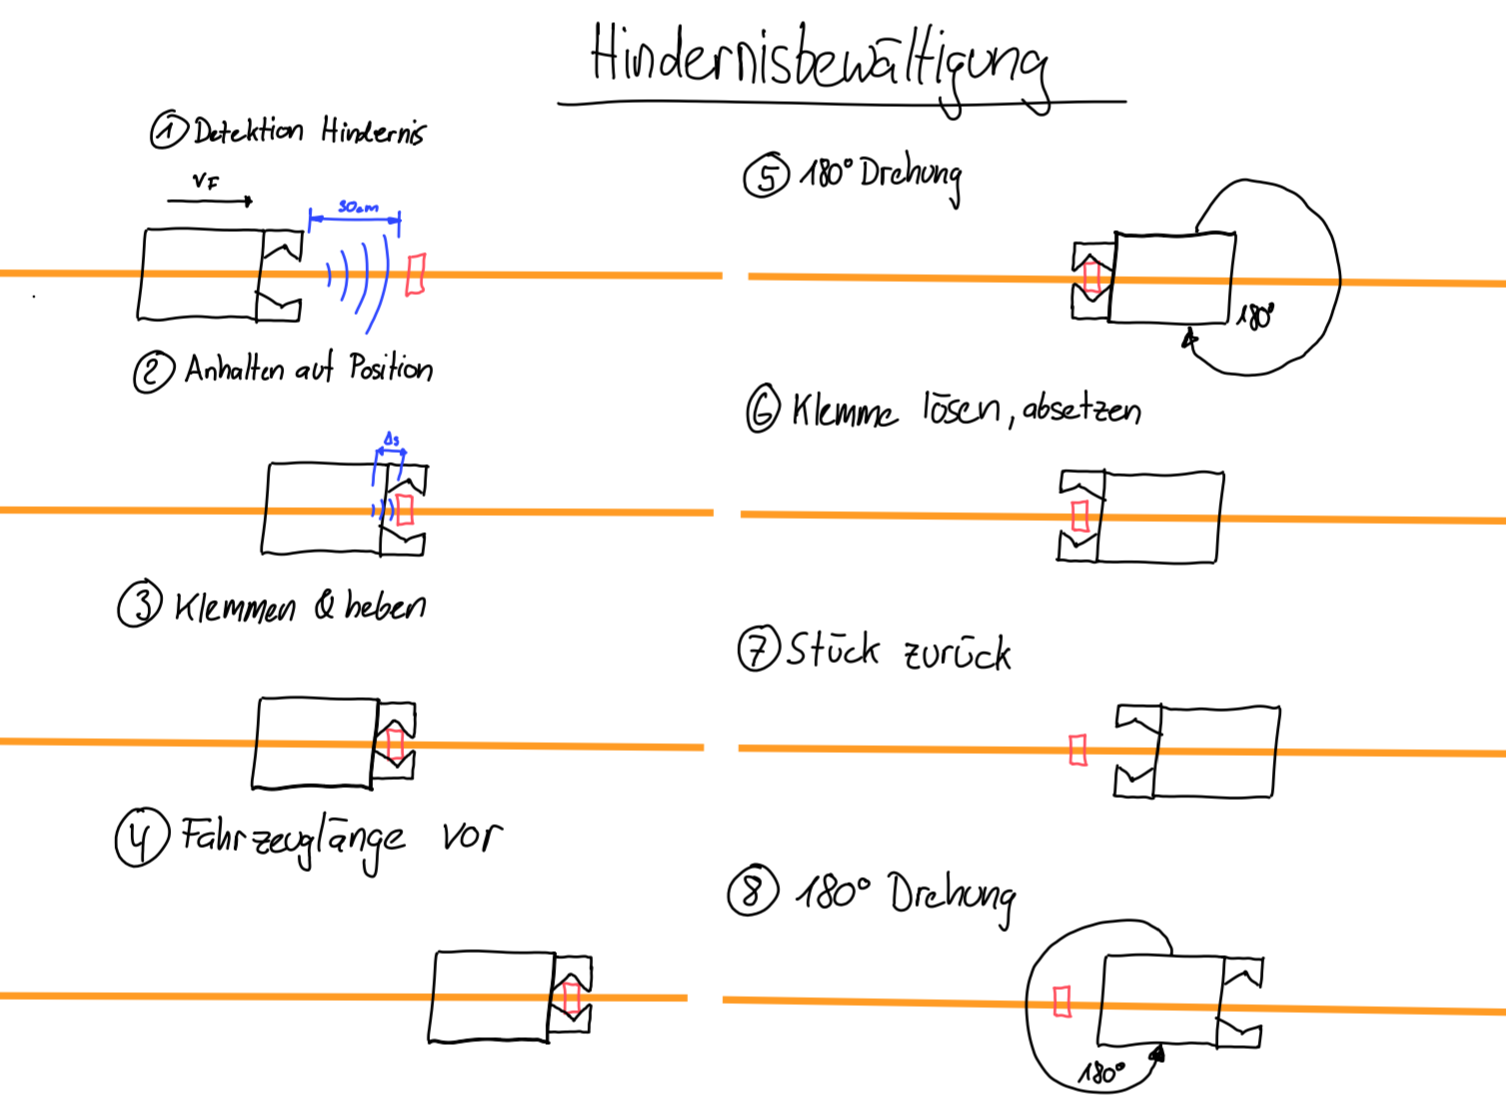
\includegraphics[width=0.8\textwidth]{img/lösungskonzpet/Skizzen/Skizze_Hindernisbewältigung.png}
\caption{Hindernisbewältigung}
\label{img:Skizze_Hindernisbewältigung}
\end{figure}

\newpage

\subsection{Energiequelle}
Aus der Technologierecherche hat sich herausgestellt, dass der LiPo-Akku der am besten geeignete Akku im Vergleich zu Li-Ion- und NiMH-Akkus ist. Dies liegt insbesondere an seiner höheren Leistungsdichte, besseren Leistungsabgabe und der Flexibilität in der Formgebung. Weitere Details dazu können im Anhang unter  \ref{a3:Energiequelle} nachgelesen werden.










% Alter Teil===========================================================================================================================================================




\subsubsection{Streckenerkennung Kamera}

TODO: Gian
- Wegpunkt wird mittels Objekterkennung erkannt (siehe ref)
- Linien bei Wegpunkt erkennen
  - Canny Edge Detection (Technologierecherche)
  - Hough Line Transform







\end{document}